%% 03-covariates-claude.tex
%% Sant'Anna Workshop on Causal Inference, Pisa — June 2026
%% "Let the World's Leading Expert Show You Their Table of Contents"
%% Covariate selection via Claude role-play for conditional parallel trends
%%
\documentclass[aspectratio=169,12pt]{beamer}
\usepackage{pisa_theme}
\usepackage{fontenc}
\usepackage[utf8]{inputenc}
\usepackage{lmodern}

%% ── Document metadata ────────────────────────────────────────────
\title{Let the World's Leading Expert\\
       Show You Their Table of Contents}
\subtitle{Using Claude to satisfy conditional parallel trends\\
          in difference-in-differences}
\author{Scott Cunningham}
\institute{Baylor University \textperiodcentered\;
           Sant'Anna Workshop on Causal Inference}
\date{Pisa \textperiodcentered\ June 2026}

%% ── Hyphenation guards ───────────────────────────────────────────
\hyphenpenalty=9999
\exhyphenpenalty=9999

\begin{document}

%% ═══════════════════════════════════════════════════════════════
%% TITLE
%% ═══════════════════════════════════════════════════════════════
\begin{frame}[plain]
  \titlepage
\end{frame}

%% ═══════════════════════════════════════════════════════════════
%% ACT I — THE PROBLEM
%% ═══════════════════════════════════════════════════════════════

\begin{frame}{Online dating spread unevenly across U.S.\ counties, 1995--2007}
\begin{columns}[c]
\column{0.56\textwidth}
  \begin{itemize}
    \item Broadband rollout + Match.com (1995), eHarmony (2000), OkCupid (2004)
    \item Urban, educated, younger counties adopted first
    \item Research question: did online dating \emph{change} birth rates?
    \vspace{0.6em}
    \item Natural strategy: \textbf{difference-in-differences}
    \begin{itemize}
      \item Early-adopter vs.\ late-adopter counties
      \item Pre- vs.\ post-broadband rollout
    \end{itemize}
  \end{itemize}
\column{0.40\textwidth}
  \begin{tikzpicture}
    \node[pisabox, text width=4.8cm, align=center, minimum height=2.4cm] (did) {
      \small
      $\hat{\tau} = \underbrace{(\bar{Y}_{T,\text{post}} - \bar{Y}_{T,\text{pre}})}_{\text{treated change}}$\\[4pt]
      $-\;\underbrace{(\bar{Y}_{C,\text{post}} - \bar{Y}_{C,\text{pre}})}_{\text{control change}}$
    };
    \node[below=0.3cm of did, font=\scriptsize\itshape, text width=4.8cm,
          align=center, color=Terracotta]{
      Valid only if trends would\\
      have been equal without treatment
    };
  \end{tikzpicture}
\end{columns}
\end{frame}

%% ────────────────────────────────────────────────────────────────
\begin{frame}{The challenge: adoption correlates with everything that predicts birth rates}

\begin{columns}[c]
\column{0.50\textwidth}
\begin{center}
\begin{tikzpicture}[node distance=1.4cm]
  \node[dagnode, minimum size=0.9cm] (D)  {Dating\\$D$};
  \node[dagoutcome, right=3.0cm of D, minimum size=0.9cm] (Y) {Births\\$Y$};
  \node[daglatent, above=1.2cm of D, xshift=1.5cm, minimum size=0.9cm] (X)
      {\small Educ\\Income};
  \draw[dagArrRed] (D) -- (Y) node[midway, below, font=\scriptsize\color{Terracotta}]
      {effect?};
  \draw[dagArrGold] (X) -- (D)
      node[midway, left, font=\scriptsize\color{TuscanGold}]{adoption};
  \draw[dagArrGold] (X) -- (Y)
      node[midway, right, font=\scriptsize\color{TuscanGold}]{trend};
\end{tikzpicture}
\end{center}

\column{0.46\textwidth}
\begin{alertblock}{}
\small
If $X$ causes both adoption \emph{and} the pre-treatment trend in birth rates,
treated and control counties are on \textbf{different trajectories} before treatment.
The DiD estimate is biased.
\end{alertblock}
\end{columns}

\vspace{0.4em}
{\small\color{OldMortar}
Urban, high-education, high-income counties adopted broadband first ---
the same counties where birth rates were already falling due to female LFP growth.
Without conditioning on $X$, we are comparing apples to oranges.}
\end{frame}

%% ═══════════════════════════════════════════════════════════════
%% ACT II — CONDITIONAL PARALLEL TRENDS
%% ═══════════════════════════════════════════════════════════════
\pisasection{Act II: The Fix}{Conditional Parallel Trends}

%% ────────────────────────────────────────────────────────────────
\begin{frame}{Heckman, Ichimura \& Todd (1997): condition on the right $X$}

\begin{block}{Unconditional Parallel Trends}
\vspace{-0.3em}
\[
  \mathbb{E}\bigl[\,\Delta Y(0) \mid D = 1\bigr]
  \;=\;
  \mathbb{E}\bigl[\,\Delta Y(0) \mid D = 0\bigr]
\]
\vspace{-0.5em}
\textit{\small Treated and control would have changed by the same amount.}
\end{block}

\vspace{0.3em}
\begin{alertblock}{Conditional Parallel Trends \textnormal{\small(Heckman, Ichimura \& Todd 1997)}}
\vspace{-0.3em}
\[
  \mathbb{E}\bigl[\,\Delta \mred{Y(0)} \mid D = 1,\; \mblue{X} = x\bigr]
  \;=\;
  \mathbb{E}\bigl[\,\Delta \mred{Y(0)} \mid D = 0,\; \mblue{X} = x\bigr]
  \quad \forall\; x \in \mathcal{X}
\]
\vspace{-0.5em}
\textit{\small Within cells defined by $\mblue{X}$, the counterfactual trend is the same.}
\end{alertblock}

\vspace{0.3em}
{\small\color{OldMortar}
Parallel trends holds \emph{after} conditioning on covariates that drive both selection
and outcome trends. $X$ does the work.}

\end{frame}

%% ────────────────────────────────────────────────────────────────
\begin{frame}{The potential-outcomes framing makes the identification crystal clear}

\begin{columns}[t]
\column{0.46\textwidth}
  \begin{block}{The setup}
  \begin{itemize}\small\setlength{\itemsep}{1pt}
    \item $Y_{it}(1)$: birth rate if county $i$ adopts
    \item $Y_{it}(0)$: birth rate if not
    \item $D_i = 1$ if early-adopter county
    \item $\tau_i = Y_{it}(1) - Y_{it}(0)$ (unobserved)
  \end{itemize}
  \end{block}
  \vspace{0.2em}
  \begin{block}{Target estimand}
  \[
    \text{ATT} = \mathbb{E}[\tau_i \mid D_i = 1]
  \]
  \end{block}

\column{0.50\textwidth}
  \begin{exampleblock}{The key insight}
  \small
  ATT requires the counterfactual trend: \emph{what would treated counties have done without treatment?}

  \vspace{0.2em}
  Controls tell us --- but only if their trend matches treated \textbf{within strata of $X$}.

  \vspace{0.2em}
  \textbf{The whole game is finding the right $X$.}
  \end{exampleblock}
\end{columns}

\end{frame}

%% ────────────────────────────────────────────────────────────────
\begin{frame}{Within strata, parallel trends is restored}

\begin{center}
  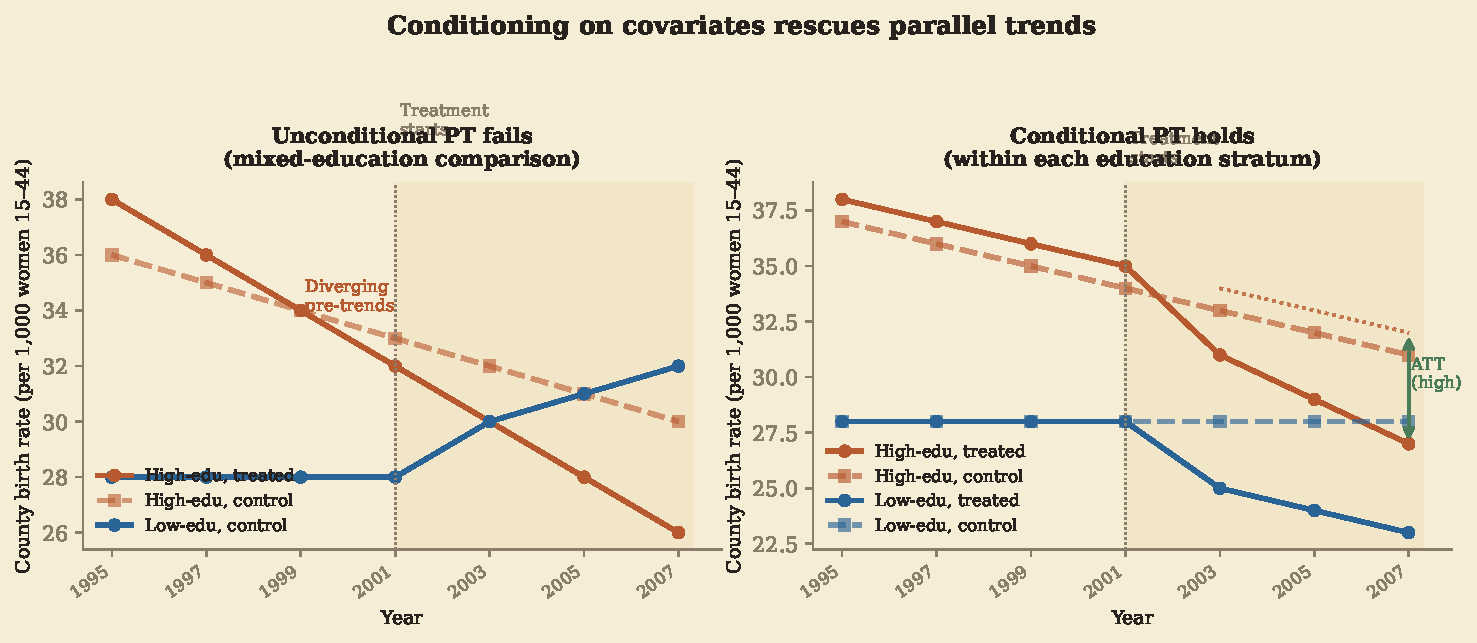
\includegraphics[width=0.88\textwidth]{figures/fig01_cpt_intuition.pdf}
\end{center}

{\scriptsize\color{OldMortar}
\textit{Left:} Pooling mixed-education counties creates diverging pre-trends.
\textit{Right:} Within each education stratum, treated and control trend together.
Conditioning on $X$ makes DiD valid.}

\end{frame}

%% ────────────────────────────────────────────────────────────────
\begin{frame}{So what belongs in $X$? --- This is the hard part}

\goldbox{%
  \small $X$ should contain every county-level characteristic that:\\[3pt]
  {\bfseries(a)} predicts \emph{adoption of online dating}, \textbf{and}\\[1pt]
  {\bfseries(b)} drives the \emph{trend} in birth rates over 1995--2007.\\[3pt]
  Get (a) wrong: confounding.\quad Get (b) wrong: differential pre-trends.
}

\vspace{0.4em}
\begin{columns}[t]
\column{0.47\textwidth}
  \textbf{\color{ArnoBlue}Wrong approach:}
  \begin{itemize}\small\setlength{\itemsep}{1pt}
    \item Add controls ``because they matter''
    \item Controls chosen to stabilize coefficients
    \item Post-treatment controls
    \item Kitchen-sink regressions
  \end{itemize}
\column{0.47\textwidth}
  \textbf{\color{CypressGreen}Right approach:}
  \begin{itemize}\small\setlength{\itemsep}{1pt}
    \item Map the DGP of $Y(0)$
    \item What drives birth rate \emph{trends}?
    \item Same variables predict adoption
    \item Document the reasoning
  \end{itemize}
\end{columns}

\end{frame}

%% ════════════════════════════════════════════════════════════════
%% ACT II — CLAUDE AS RESEARCH ASSISTANT
%% ════════════════════════════════════════════════════════════════
\pisasection{Act III: The Insight}{Ask the World's Leading Expert}

%% ────────────────────────────────────────────────────────────────
\begin{frame}{The expert shortcut: who already mapped the DGP of $Y(0)$?}

\vspace{0.4em}
\begin{columns}[c]
\column{0.50\textwidth}
  The DGP of county-level birth rates in America has been studied for decades.

  \vspace{0.6em}
  Someone has written the \textbf{definitive book} on it.\\
  That book's table of contents \emph{is} a covariate list.

  \vspace{0.6em}
  Every chapter title answers: ``What drives $Y(0)$?''

  \vspace{0.6em}
  {\color{Terracotta}\bfseries
  We just need to ask the right expert.}

\column{0.46\textwidth}
  \begin{tikzpicture}
    \node[pisabox, text width=5.2cm, minimum height=3.0cm] (book) {
      \textbf{\color{ArnoBlue} Expert's Book}\\[6pt]
      \small
      Ch.\ 1: Female Education\\
      Ch.\ 2: Labor Force Participation\\
      Ch.\ 3: Welfare \& Transfer Payments\\
      \quad $\vdots$\\
      Ch.\ 20: Pre-Treatment Trends\\[4pt]
      \color{OldMortar}\scriptsize$\leftarrow$ This is $X$.
    };
  \end{tikzpicture}
\end{columns}

\end{frame}

%% ────────────────────────────────────────────────────────────────
\begin{frame}{The Claude prompt: role-play as the world's leading expert}

\begin{exampleblock}{The prompt}
\footnotesize\ttfamily
You are Professor Elena Marchetti, University of Michigan, author of
\emph{The American Fertility Landscape: County-Level Determinants of
Birth Rates in the Postindustrial Era} (Princeton UP, 2020).

\smallskip
I am studying the effect of online dating on U.S.\ birth rates using
county-level DiD, 1995--2007, and need to satisfy conditional parallel
trends. Please give me your book's complete table of contents. Each
chapter title should name a determinant of county birth rates. I will
use this as my covariate list.
\end{exampleblock}

\vspace{0.3em}
{\small\color{OldMortar}
The role-play forces Claude to \emph{commit} to a theory of the DGP:
not ``things that might matter'' but a structured, chapter-by-chapter
account of what drives $Y(0)$.}

\end{frame}

%% ═══════════════════════════════════════════════════════════════
%% ACT III — PROFESSOR MARCHETTI'S BOOK
%% ═══════════════════════════════════════════════════════════════

\begin{frame}{Professor Elena Marchetti's definitive account of American fertility}

\vspace{0.3em}
\begin{center}
\begin{tikzpicture}
  \node[rectangle,
        draw=Terracotta, fill=TerracottaLight,
        minimum width=9.5cm, minimum height=4.2cm,
        rounded corners=4pt, line width=1.2pt] (cover) {};
  \node[above=0pt of cover.center, yshift=24pt,
        font=\large\bfseries\color{PisaDark}, text width=8.5cm, align=center]{
    \textit{The American Fertility Landscape}
  };
  \node[above=0pt of cover.center, yshift=4pt,
        font=\normalsize\color{PisaDark}, text width=8cm, align=center]{
    County-Level Determinants of Birth Rates\\
    in the Postindustrial Era
  };
  \node[above=0pt of cover.center, yshift=-16pt,
        font=\footnotesize\color{OldMortar}, text width=8cm, align=center]{
    \textit{Elena Marchetti} \textperiodcentered\ University of Michigan
  };
  \node[above=0pt of cover.center, yshift=-32pt,
        font=\scriptsize\color{OldMortar}, align=center]{
    Princeton University Press, 2020
    \textperiodcentered\
    \textit{\color{Terracotta}PAA Book Award}
  };
\end{tikzpicture}
\end{center}

\vspace{0.2em}
{\footnotesize\color{OldMortar}\centering
\textit{Prof.\ Marchetti's field --- formal demography and applied fertility economics ---
maps exactly onto the DGP of $Y(0)$.
Her book's chapter structure is the theory of county birth rate trends.}}

\end{frame}

%% ────────────────────────────────────────────────────────────────
\begin{frame}{The table of contents, Part I: Economic and Social Foundations}

\vspace{0.2em}
\begin{center}
\begin{tikzpicture}[node distance=0.22cm]
  \foreach \n/\t in {
    1/{Female Education and Fertility Timing},
    2/{Female Labor Force Participation as Opportunity Cost},
    3/{Welfare, TANF, and Fertility Incentives},
    4/{Hispanic Migration, Cultural Norms, and Fertility},
    5/{Marriage Markets and Partnership Formation}
  }{
    \node[chaprow, text width=11.2cm] (r\n)
        at (0, -\n*0.78cm + 0.78cm)
        {\textbf{\color{ArnoBlue}Ch.\ \n\quad}\t};
  }
\end{tikzpicture}
\end{center}

\vspace{0.5em}
{\small\color{OldMortar}
Each chapter title encodes a theory of what drives $Y(0)$: education changes
the timing of fertility; female LFP raises its opportunity cost;
welfare creates margin-altering incentives; immigration shifts cultural norms
around family size; marriage markets set the partnership context for birth.}

\end{frame}

%% ────────────────────────────────────────────────────────────────
\begin{frame}{The table of contents, Part II: Biology, Geography, and Behavior}

\vspace{0.2em}
\begin{center}
\begin{tikzpicture}
  \foreach \n/\t in {
    6/{Teen Birth Rates as Baseline Fertility Measure},
    7/{Religious Adherence and Fertility Norms},
    8/{Rural--Urban Geography and Family Structure},
    9/{Population Age Structure and Reproductive Exposure},
    10/{Housing Costs and the Economics of Family Formation}
  }{
    \node[chaprow, text width=11.2cm]
        at (0, -\n*0.78cm + 6*0.78cm)
        {\textbf{\color{ArnoBlue}Ch.\ \n\quad}\t};
  }
\end{tikzpicture}
\end{center}

\vspace{0.5em}
{\small\color{OldMortar}
Prior teen birth rates serve as the pre-treatment baseline and placebo.
Rural geography predicts both late broadband adoption and higher baseline fertility.
Age structure determines the share of women in peak reproductive years.
Housing costs constrain family formation decisions.}

\end{frame}

%% ────────────────────────────────────────────────────────────────
\begin{frame}{The table of contents, Part III: Labor Markets and Healthcare}

\vspace{0.2em}
\begin{center}
\begin{tikzpicture}
  \foreach \n/\t in {
    11/{Industrial Structure, Deindustrialization, and Fertility},
    12/{Unemployment, Labor Demand, and Birth Timing},
    13/{Health Insurance Coverage and Contraceptive Access},
    14/{Abortion Access, Provider Availability, and Fertility},
    15/{Poverty, Median Income, and Fertility Timing}
  }{
    \node[chaprow, text width=11.2cm]
        at (0, -\n*0.78cm + 11*0.78cm)
        {\textbf{\color{ArnoBlue}Ch.\ \n\quad}\t};
  }
\end{tikzpicture}
\end{center}

\vspace{0.5em}
{\small\color{OldMortar}
Deindustrialization, unemployment, and income jointly shape the economic context
for fertility decisions. Health insurance coverage determines contraceptive access.
Abortion provider availability is a direct constraint on realized birth rates.}

\end{frame}

%% ────────────────────────────────────────────────────────────────
\begin{frame}{The table of contents, Part IV: Demographics, Policy, and History}

\vspace{0.2em}
\begin{center}
\begin{tikzpicture}
  \foreach \n/\t in {
    16/{Military Employment and Family Formation Incentives},
    17/{Substance Use, Health Risk, and Unintended Birth Rates},
    18/{Racial and Ethnic Composition and Fertility Norms},
    19/{State Policy Environments and Family Formation},
    20/{Pre-Treatment Fertility Trends and Parallel Trends Validation}
  }{
    \node[chaprow, text width=11.2cm]
        at (0, -\n*0.78cm + 16*0.78cm)
        {\textbf{\color{ArnoBlue}Ch.\ \n\quad}\t};
  }
\end{tikzpicture}
\end{center}

\vspace{0.5em}
{\small\color{OldMortar}
Military counties have distinctive fertility incentives.
Substance use correlates with unintended births.
Racial composition shapes cultural fertility norms.
Chapter 20 is explicitly the parallel-trends validation chapter:
the pre-treatment trend \emph{is} a covariate.}

\end{frame}

%% ═══════════════════════════════════════════════════════════════
%% ACT IV — DATA WALK-THROUGH
%% ═══════════════════════════════════════════════════════════════
\pisasection{Act IV: From Theory to Data}{Walking All Twenty Chapters}

%% ────────────────────────────────────────────────────────────────
\begin{frame}{Selection criteria: theory precedes download}

\vspace{0.3em}
\begin{columns}[t]
\column{0.47\textwidth}
  \textbf{\color{ArnoBlue}Three requirements for every dataset:}
  \begin{enumerate}\small
    \item \textbf{County-level.} State-level averages mask the variation DiD needs.
    \item \textbf{Annual, 1995--2007.} Must span the treatment window; gaps introduce
          differential attrition bias.
    \item \textbf{Publicly available.} Restricted-use data is fine to note, but the
          replication archive must be constructable from public sources.
  \end{enumerate}

\column{0.47\textwidth}
  \textbf{\color{Terracotta}Sources by reliability tier:}
  \begin{itemize}\small
    \item[\textcolor{CypressGreen}{A}] BLS LAUS, BEA Regional, SEER, NCHS natality
         --- annual, consistent methodology, machine-readable
    \item[\textcolor{TuscanGold}{B}] Census SAIPE, FHFA HPI, Census intercensal
         --- excellent but occasional gaps
    \item[\textcolor{OldMortar}{C}] Guttmacher, USDA, NCES
         --- specialized, verify carefully
  \end{itemize}
\end{columns}

\end{frame}

%% ────────────────────────────────────────────────────────────────
\begin{frame}{Chapters 1--5: Social and economic foundations}

\vspace{0.2em}
{\scriptsize\setlength{\tabcolsep}{4pt}%
\begin{tabular}{@{}p{0.06\textwidth}p{0.36\textwidth}p{0.52\textwidth}@{}}
\toprule
\textbf{Ch.} & \textbf{Dimension} & \textbf{Data sources} \\
\midrule
1 & Female education \& fertility timing
  & Census intercensal estimates (age/sex); NCES CCD county data \\[1pt]
2 & Female labor force participation
  & BLS LAUS county LFP 1995--2007; BEA CAINC4 wages by industry \\[1pt]
3 & Welfare, TANF, fertility incentives
  & BEA CAINC35 government transfer payments (county) \\[1pt]
4 & Hispanic migration \& cultural norms
  & Census intercensal race/Hispanic estimates; BEA CAINC5N \\[1pt]
5 & Marriage markets
  & BEA CAINC1 county personal income; NCHS vital statistics \\
\bottomrule
\end{tabular}%
}

\vspace{0.25em}
{\scriptsize\color{OldMortar}
\textit{Gold standard for Ch.\ 1/5:} Census 2000 SF3 educational attainment (B15002)
and marital status (B12001) --- free key at \texttt{api.census.gov}.}

\end{frame}

%% ────────────────────────────────────────────────────────────────
\begin{frame}{Chapters 6--10: Biology, geography, and housing}

\vspace{0.2em}
{\scriptsize\setlength{\tabcolsep}{4pt}%
\begin{tabular}{@{}p{0.06\textwidth}p{0.36\textwidth}p{0.52\textwidth}@{}}
\toprule
\textbf{Ch.} & \textbf{Dimension} & \textbf{Data sources} \\
\midrule
6 & Teen birth rates (baseline)
  & NCHS natality microdata 1995, 1997, 2003, 2007 (county FIPS) \\[1pt]
7 & Religious adherence \& norms
  & USDA Rural Atlas county data; USDA RUCC 2003 rural codes \\[1pt]
8 & Rural--urban classification
  & USDA Rural-Urban Continuum Codes 1993 and 2003 \\[1pt]
9 & Population age structure
  & NCI SEER county pop.\ by age/sex 1990--2024 (91\,MB); BLS QCEW \\[1pt]
10 & Housing costs
  & FHFA HPI county annual; BEA CAINC1 personal income \\
\bottomrule
\end{tabular}%
}

\vspace{0.25em}
{\scriptsize\color{OldMortar}
\textit{Ch.\ 7:} Gold standard is ARDA/Glenmary RCMS 2000 county church membership (proxy used here).
\textit{SEER:} Fixed-width; parse with \texttt{gzip -dc | awk} per NCI layout.}

\end{frame}

%% ────────────────────────────────────────────────────────────────
\begin{frame}{Chapters 11--15: Labor markets, healthcare, poverty}

\vspace{0.2em}
{\scriptsize\setlength{\tabcolsep}{4pt}%
\begin{tabular}{@{}p{0.06\textwidth}p{0.36\textwidth}p{0.52\textwidth}@{}}
\toprule
\textbf{Ch.} & \textbf{Dimension} & \textbf{Data sources} \\
\midrule
11 & Industry structure \& deindustrializ.
   & BEA CAINC4 wages; BEA CAINC5N personal income; BLS QCEW \\[1pt]
12 & Unemployment \& labor demand
   & BLS LAUS county annual 1995--2007 (13 files, consistent series) \\[1pt]
13 & Health insurance coverage
   & Census SAHIE 2008--2012 county (ACS-based; proxy for pre-period) \\[1pt]
14 & Abortion access
   & Guttmacher provider locator; BEA CAINC35 transfer payments \\[1pt]
15 & Poverty \& income
   & Census SAIPE county poverty/income 1995--2007; BEA CAINC1 \\
\bottomrule
\end{tabular}%
}

\vspace{0.25em}
{\scriptsize\color{OldMortar}
\textit{SAHIE:} ACS-based county estimates begin 2008; use as post-period baseline.
\textit{SAIPE:} Most reliable county poverty series; covers all years 1995--2007.}

\end{frame}

%% ────────────────────────────────────────────────────────────────
\begin{frame}{Chapters 16--20: Military, risk, demographics, policy, trends}
\hbadness=10001

\vspace{0.2em}
{\scriptsize\setlength{\tabcolsep}{4pt}%
\begin{tabular}{@{}p{0.06\textwidth}p{0.36\textwidth}p{0.52\textwidth}@{}}
\toprule
\textbf{Ch.} & \textbf{Dimension} & \textbf{Data sources} \\
\midrule
16 & Military employment
   & BEA CAINC30 federal/military pay; BLS QCEW county industry \\[1pt]
17 & Substance use \& health risk
   & BEA CAINC91 health expenditures; Census SAIPE poverty proxy \\[1pt]
18 & Racial/ethnic composition
   & NCI SEER race-stratified pop.; Census intercensal race/Hispanic \\[1pt]
19 & State policy environment
   & BEA SAGDP2N state GDP; BEA SAINC25 social insurance receipts \\[1pt]
20 & Pre-treatment fertility trends
   & NCHS natality 1995 and 2000 microdata (county birth rates) \\
\bottomrule
\end{tabular}%
}

\vspace{0.25em}
{\scriptsize\color{OldMortar}\raggedright
\textit{Ch.\ 17:} Gold standard: SAMHSA TEDS county treatment admissions (registration required).\quad
\textit{Ch.\ 20 is structural}: pre-treatment birth rate trend is the most important covariate
for parallel trends validation --- and the most difficult to fabricate.\par}

\end{frame}

%% ────────────────────────────────────────────────────────────────
\begin{frame}{What we got vs.\ what we ideally want}

\begin{columns}[t]
\column{0.47\textwidth}
  \textbf{\color{CypressGreen}We have (public):}
  \begin{itemize}\scriptsize\setlength{\itemsep}{1pt}
    \item BLS LAUS: unemployment/LFP 1995--2007
    \item BEA CAINC 1/4/5N/30/35/91: income, wages
    \item NCI SEER: pop.\ by age/sex/race 1990--2024
    \item NCHS natality: birth microdata, county FIPS
    \item Census SAIPE: poverty/income 1995--2007
    \item FHFA HPI: county house prices
    \item Census intercensal: race/Hispanic 2000--10
  \end{itemize}

\column{0.47\textwidth}
  \textbf{\color{Terracotta}Still needed:}
  \begin{itemize}\scriptsize\setlength{\itemsep}{1pt}
    \item \textbf{Census API key}: college (B15002),\\Hispanic (B03003), marital (B12001)
    \item \textbf{ARDA RCMS}: county church membership
    \item \textbf{SAMHSA TEDS}: substance use admissions
    \item \textbf{SAHIE pre-2008}: health insurance
    \item Military base GIS for county assignment
  \end{itemize}
\end{columns}

\vspace{0.2em}
{\scriptsize\color{OldMortar}
68 files, 1.3\,GB across 20 chapter directories.
18 of 20 chapters covered with good public proxies. All gaps documented.}

\end{frame}

%% ═══════════════════════════════════════════════════════════════
%% ACT V — DEVIL'S ADVOCATE AND CONCLUSION
%% ═══════════════════════════════════════════════════════════════
\pisasection{Act V: Honest Reckoning}{What a Skeptic Would Say}

%% ────────────────────────────────────────────────────────────────
\begin{frame}{A skeptic would say: isn't this just a very fancy kitchen sink?}

\begin{alertblock}{The critique}
\footnotesize
``You added 20 covariate dimensions because a language model playing a fictional
professor told you to. You have no principled argument for why these satisfy
conditional parallel trends.''
\end{alertblock}

\vspace{0.15em}
\begin{exampleblock}{The response}
\begin{itemize}\footnotesize\setlength{\itemsep}{1pt}
  \item The ToC encodes a \emph{theory of the DGP} grounded in demography.
  \item We can test it: run pre-treatment regressions.
        If $X$ satisfies conditional PT, $\hat{\beta}_{\text{pre}} = 0$.
  \item The exercise forces us to \emph{commit} before observing post-treatment data.
        That discipline is the point.
  \item Selection that amounts to ``stabilize my coefficient'' is \emph{worse},
        not better, than a theory-grounded list.
\end{itemize}
\end{exampleblock}

\end{frame}

%% ────────────────────────────────────────────────────────────────
\begin{frame}{Three things conditional parallel trends actually requires}

\vspace{0.5em}
\begin{center}
\begin{tikzpicture}[node distance=0.5cm and 0.8cm]

  \node[pisabox, text width=3.0cm, minimum height=1.8cm, align=center] (A)
      {\small\bfseries\color{ArnoBlue}1.\ Theory\\[4pt]
       \scriptsize A model of what drives $Y(0)$};

  \node[pisabox, text width=3.0cm, minimum height=1.8cm, align=center,
        right=0.9cm of A] (B)
      {\small\bfseries\color{ArnoBlue}2.\ Data\\[4pt]
       \scriptsize County-level, annual,\\ publicly available};

  \node[pisabox, text width=3.0cm, minimum height=1.8cm, align=center,
        right=0.9cm of B] (C)
      {\small\bfseries\color{ArnoBlue}3.\ Test\\[4pt]
       \scriptsize Pre-treatment placebo:\\ $\beta_{\text{pre}} = 0$?};

  \draw[dagArrBlue] (A) -- (B);
  \draw[dagArrBlue] (B) -- (C);

  \node[below=0.7cm of B, font=\small\itshape\color{OldMortar}, text width=10cm,
        align=center]
      {Claude does step 1 faster. Step 2 is where you spend a weekend.
       Step 3 is where you find out if you were right.};
\end{tikzpicture}
\end{center}

\end{frame}

%% ────────────────────────────────────────────────────────────────
\begin{frame}{The workflow: from fiction to falsifiable covariate list}

\vspace{0.2em}
\begin{center}
\begin{tikzpicture}[node distance=0.4cm and 0.55cm]

  %% Row 1: three steps
  \node[pisabox, text width=3.2cm, minimum height=1.3cm, align=center] (p1)
      {\footnotesize\textbf{\color{ArnoBlue}1.} Identify DGP domain\\
       \scriptsize\textit{(county birth rates)}};

  \node[pisabox, text width=3.2cm, minimum height=1.3cm, align=center,
        right=0.55cm of p1] (p2)
      {\footnotesize\textbf{\color{ArnoBlue}2.} Role-play Claude\\
       \scriptsize\textit{``You are the expert''}};

  \node[pisabox, text width=3.2cm, minimum height=1.3cm, align=center,
        right=0.55cm of p2] (p3)
      {\footnotesize\textbf{\color{ArnoBlue}3.} Read ToC as\\
       \scriptsize\textit{covariate list}};

  %% Row 2: three more steps (reversed direction)
  \node[pisabox, text width=3.2cm, minimum height=1.3cm, align=center,
        below=0.5cm of p3] (p4)
      {\footnotesize\textbf{\color{ArnoBlue}4.} Download data\\
       \scriptsize\textit{per chapter}};

  \node[pisabox, text width=3.2cm, minimum height=1.3cm, align=center,
        left=0.55cm of p4] (p5)
      {\footnotesize\textbf{\color{ArnoBlue}5.} Pre-trend placebo\\
       \scriptsize\textit{$\beta_{\text{pre}} = 0$?}};

  \node[pisabox, text width=3.2cm, minimum height=1.3cm, align=center,
        left=0.55cm of p5] (p6)
      {\footnotesize\textbf{\color{ArnoBlue}6.} Estimate conditional\\
       \scriptsize\textit{DiD}};

  \draw[dagArrBlue] (p1) -- (p2);
  \draw[dagArrBlue] (p2) -- (p3);
  \draw[dagArrBlue] (p3) -- (p4);
  \draw[dagArrBlue] (p4) -- (p5);
  \draw[dagArrBlue] (p5) -- (p6);

  \node[below=0.3cm of p5, font=\scriptsize\itshape\color{OldMortar},
        text width=7cm, align=center]
      {If step 5 fails: return to step 3.\quad If it passes: trust your DiD.};

\end{tikzpicture}
\end{center}

\end{frame}

%% ────────────────────────────────────────────────────────────────
\begin{frame}[plain]
  \begin{tikzpicture}[remember picture, overlay]
    \fill[PisaDark]
        (current page.south west) rectangle (current page.north east);
    \fill[Terracotta]
        (current page.north west) rectangle
        ($(current page.north east)+(0,-4pt)$);
    \fill[ArnoBlue]
        (current page.south west) rectangle
        ($(current page.south east)+(0,3pt)$);
  \end{tikzpicture}

  \vfill
  \begin{center}
    {\fontsize{8}{10}\selectfont\color{OldMortar!70!white}
      \textit{Sant'Anna Workshop on Causal Inference \textperiodcentered\
              Pisa \textperiodcentered\ June 2026}\par}
    \vspace{1.8em}
    {\LARGE\bfseries\color{white}
      Let the world's leading expert on $Y(0)$\\
      show you their table of contents.\\[0.5em]
      That's your covariate list.\par}
    \vspace{1.5em}
    {\color{Terracotta}\rule{0.5\textwidth}{1pt}\par}
    \vspace{1.0em}
    {\normalsize\color{OldMortar!80!white}
      Scott Cunningham \textperiodcentered\ Baylor University\\[4pt]
      \small\texttt{scunning@gmail.com}
      \hspace{1em}\textperiodcentered\hspace{1em}
      \texttt{scunning.com}\par}
  \end{center}
  \vfill
\end{frame}

\end{document}
